\documentclass[10pt,a4paper]{article}
\usepackage[a4paper, top=2cm, bottom=1.5cm, left=1.5cm, right=1.5cm]{geometry} % Задать размеры полей.
\usepackage[warn]{mathtext} % Русские символы в формулах. Нужно писать до пакета babel. Указывает, что в формулах используются символы кириллицы, которые по умолчанию печатаются прямым шрифтом.
\usepackage[T2A]{fontenc}
\usepackage[utf8]{inputenc}
\usepackage[russian]{babel}
\usepackage{amsmath}
\usepackage{amssymb}
\usepackage{graphicx}
%\usepackage{floatrow}
\usepackage{booktabs}
\usepackage{wrapfig}
\usepackage{fancyhdr}
\usepackage{multicol}
\usepackage{xcolor}

\usepackage{float}
\usepackage{multirow}

\newcommand{\figref}[1]{(См. рис. \ref{#1})}
\newcommand{\secref}[1]{(См. раздел. \ref{#1})}

\newcommand{\e}[1]{\text{$\cdot10^{#1}$}}
\newcommand{\m}{\; м}
\newcommand{\mm}{\; мм}
\newcommand{\um}{\; мкм}
\newcommand{\A}{\; А}
\newcommand{\uV}{\; мкВ}
\newcommand{\cels}{\; ^\circ С}

\pagestyle{fancy}
\fancyhead{}
\fancyhead[L]{\small Дедков Д.А., Маслов А.С., Измерение коэффициента ослабления потока $\gamma$-лучей в веществе и определение их энергий. МФТИ, 2023 г.}
\fancyhead[R]{}
\fancyfoot[C]{\thepage}

\renewcommand{\cot}{\text{ctg}}

\author{\normalsize Дедков Денис, Маслов Артём \\
	\normalsize группа Б01-108а \\
	\normalsize 25.09.2023}
\date{}

\title{
	\Large Измерение коэффициента ослабления потока $\gamma$-лучей в веществе и определение их энергий \\ 
}

\begin{document}
\maketitle
	
	\subsection*{Цель и задачи работы:}
	\begin{enumerate}
		\item С помощью сцинтилляционного счётчика измерить линейные коэффициенты ослабления потока $\gamma$-лучей в свинце, железе, алюминии.
		
		\item По линейным коэффициентам ослабления потока $\gamma$-лучей определить энергию $\gamma$-квантов.
	\end{enumerate}
	
	\subsection*{Описание экспериментальной установки}
	
	Схема экспериментальной установки приведена на рисунке \ref{img:exp_scheme}:
	\begin{figure}[H]
		\centering
		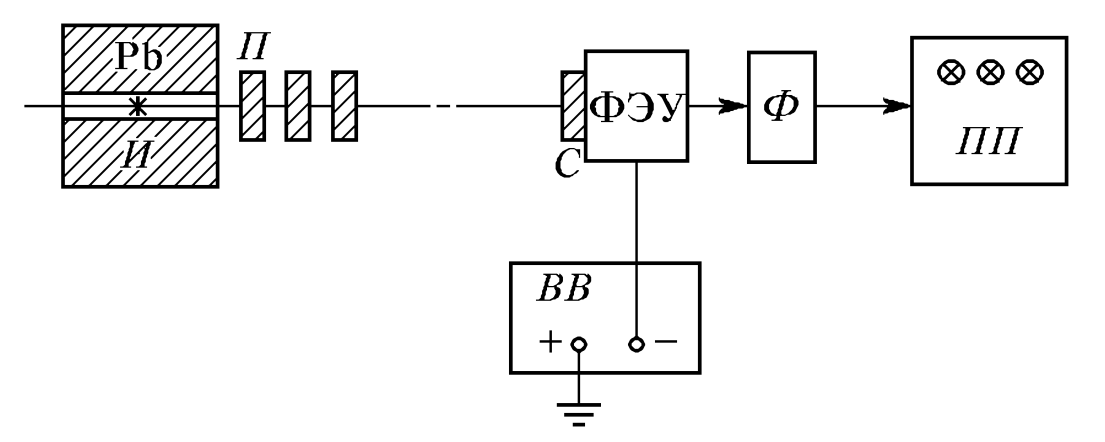
\includegraphics[width=0.5\textwidth]{images/exp_scheme.png}
		\caption{Схема экспериментальной установки.}
		\label{img:exp_scheme}
	\end{figure}

	Источник $\gamma$-лучей И окружён свинцовой оболочкой. Коллиматор выделяет узкий параллельный пучок $\gamma$-квантов, который проходит через набор поглотителей П, и регистрируется сцинтилляционным счётчиком С (кристалл $NaI(Tl)$). Сигнал со счётчика усиливается каскадом фотоэлектронного умножителя и формирователя-выпрямителя Ф, и регистрируется пересчётным прибором ПП. Высоковольтный выпрямитель ВВ обеспечивает питание сцинтилляционного счётчика.
	
	\subsection*{Оборудование и приборы}
	
	Экспериментальная установка №5.1б.
	
	\begin{enumerate}
		\item Набор поглотителей из алюминия, свинца и железа. Инвентарный номер №410134125708.
		
		\item Блок детектирования сцинтилляционный РАДЭК БДЕГ-40. Заводской номер №2914. Инвентарный номер №4024.
		
		\item Высоковольтный источник питания Scaler 1403. Инвентарный номер №410134125708.
		
		\item Источник гамма-излучения в свинцовой оболочке.
		
		\item Штангенциркуль. Погрешность измерения равна половине цены деления $\sigma_{штангенциркуль} = 0.05 \mm$.
	\end{enumerate}
	
	\subsection*{Первичные экспериментальные данные}
	
	Первичные экспериментальные данные приведены в таблицах 1-4. Погрешность измерения $L_i$ одинакова и равна $\sigma_{штангенциркуль} = 0.05 \mm$.
	
	Условные обозначения: $N$ -- число частиц попадающих на счётчик за время $T$. $L$ -- суммарная толщина поглотителя, $L_i$ -- толщина отдельных частей поглотителя.
	
	\begin{multicols}{2}
		\begin{tabular}[t]{l}
			Таблица 1. Радиационный фон. \\
			\input{gen/tab-fed1.tex}
		\end{tabular}
		
		\begin{tabular}[t]{l}
			Таблица 2. Поглотитель из свинца. \\
			\input{gen/tab-fed2.tex}
		\end{tabular} 
	\end{multicols}
	
	\begin{multicols}{2}
		\begin{tabular}[t]{l}
			Таблица 3. Поглотитель из железа. \\
			\input{gen/tab-fed3.tex}
		\end{tabular}
		
		\begin{tabular}[t]{l}
			Таблица 4. Поглотитель из алюминия. \\
			\input{gen/tab-fed4.tex}
		\end{tabular}
	\end{multicols}
	
	\subsection*{Обработка экспериментальных данных}
	
	Уровень радиационного фона определим как:
	$$
	n_{шум} = <\frac{N}{T}>
	$$
	где $<x>$ -- среднее значение $x$.
	$$\input{gen/eq-noise.tex}$$
	
	Среднеквадратичное отклонение $n_{шум}$ определялось по формуле:
	$$
	\sigma_{n_{шум}} = \sqrt{\frac{1}{k - 1} \sum_{i = 1}^{k}(n_i - <n>)^2}
	$$
	
	Построим график зависимости количества зарегистрированных в секунду $\gamma$-квантов $n$ от толщины поглощающего слоя $l$ в обычном и логарифмическом масштабе (рис. \ref{fig:nl}, \ref{fig:lnnl}).
	
	\begin{figure}[H]
		\centering
		\begin{minipage}[c]{0.48\textwidth}
			\centering
			\includegraphics[width=0.9\textwidth]{gen/fig-nl.png}
			
			\caption{График зависимости $n(l)$.}
			\label{fig:nl}
		\end{minipage}
		\hfill
		\begin{minipage}[c]{0.48\textwidth}
			\centering
			\includegraphics[width=0.9\textwidth]{gen/fig-lnnl.png}
			
			\caption{График зависимости $\ln n(l)$.}
			\label{fig:lnnl}
		\end{minipage}
	\end{figure}

	Погрешность $n$ оценивалась по формулам: \\
	\begin{center}
		$
		\sigma_n = \sqrt{\sigma_{N/t}^2 + \sigma_{n_{шум}}^2}
		$\\
		$
		\sigma_{N/t} = \frac{N}{t} \cdot \varepsilon_{N} = \frac{N}{t} \cdot \frac{\sigma_N}{N}
		$\\
		$
		\sigma_{\ln n} = \frac{1}{n} \cdot \sigma_n
		$\\
	\end{center}
	Кресты погрешности малы и на графиках не видны.
	
	С помощью метода наименьших квадратов проведём на графике в логарифмическом масштабе прямые. Коэффициенты наклона прямых: \\
	\begin{center}
	$\input{gen/eq-Pb.tex}$\\
	$\input{gen/eq-Fe.tex}$\\
	$\input{gen/eq-Al.tex}$
	\end{center}
	
	Определим линейные коэффициенты поглощения, приведённые к плотности вещества:
	$$\mu' = \frac{\mu}{\rho}$$
	
	\begin{center}
		$\mu'_Pb = 0.084 \pm 0.004 \; \frac{см^2}{г}$\\
		$\mu'_Fe = 0.069 \pm 0.001 \; \frac{см^2}{г}$\\
		$\mu'_Al = 0.073 \pm 0.001 \; \frac{см^2}{г}$\\
	\end{center}

	
	Были взяты следующие значения плотности:\\

	\begin{center}
		$\rho_{Pb} = 13.35 \; г/см^3$\\
		$\rho_{Fe} = 7.87  \; г/см^3$\\
		$\rho_{Al} = 2.70 \; г/см^3$
	\end{center}
			
	\subsection*{Обсуждение результатов и выводы}
	
	В работе были измерены линейные коэффициенты поглощения $Pb$, $Fe$, $Al$: \\
	\begin{center}
		$\input{gen/eq-Pb.tex}$\\
		$\input{gen/eq-Fe.tex}$\\
		$\input{gen/eq-Al.tex}$
	\end{center}
	
	Табличные значения линейных коэффициентов поглощения $\mu$ в $см^{-1}$:
	
	\begin{table}[H]
		\centering
		\begin{tabular}{cccc}
			\toprule
			$E_\gamma, \; МэВ$ & Al & Fe & Pb \\
			\midrule
			0.6 & 0.210 & 0.605 & 1.349 \\
			0.8 & 0.184 & 0.526 & 0.982 \\
			\bottomrule
		\end{tabular}
	\end{table}
	
	По табличным данным можно сделать вывод, что энергия измеряемых в работе гамма-квантов была в диапазоне $[0.6; 0.8] \; МэВ$.
	
\end{document}